\section{Experiments}

\subsection{Protocol and Metrics}

The experiments follow a six-link evidence chain: existence, formation attribution, matched mitigation, cross-communication replication, HFL field-position comparison, and external-validity boundaries. We report DSA together with operator-grid accuracy and frozen task metrics: client-average accuracy (Avg), minimum client accuracy (Worst), worst valid class--operator-cell accuracy (WCCA), and the mean within-class accuracy range across operators (CFG; lower is better).

The experiments use matched contrasts rather than a single cross-protocol leaderboard. The held-out map2 study is the main comparison of local risk objectives; map1 changes the class--operator binding while keeping the remaining controlled factors fixed; FedDF-fidelity changes the HFL communication base. Table~\ref{tab:protocol-boundary} summarizes the information available during training and evaluation.

\begin{table*}[t]
\centering
\small
\caption{Information boundary for completed and frozen comparison protocols. Operator identities and binding maps are sealed from deployable training.}
\label{tab:protocol-boundary}
\resizebox{\textwidth}{!}{%
\begin{tabular}{lllll}
\toprule
Protocol role & Private task & Train-time environment information & Communication context & Evaluation-only information \\
\midrule
CLE formation / local-first & CIFAR--10 & none & Local or strict AsymHFL & operator, binding, paired grid \\
Axis I strong-stress objectives ($\alpha=.5,\rho=1,\gamma=.9$) & CIFAR--10 & none or PEW family proxy, by arm & strict AsymHFL & operator, binding, paired grid \\
Cross-binding map1 & CIFAR--10 & PEW family proxy for PEW+BER & strict AsymHFL & operator, binding, paired grid \\
Second communication base & CIFAR--10 & PEW family proxy for PEW+BER & FedDF-fidelity & operator, binding, paired grid \\
Moderate dose response ($\alpha=1,\rho=.5$) & CIFAR--10 & none or PEW family proxy, by arm & strict AsymHFL & operator, binding, paired grid \\
Axis II moderate context ($\alpha=1,\rho=.5,\gamma=.9$) & CIFAR--10 & method-specific; BER only in its named row & protocol-matched HFL family & operator, binding, paired grid \\
\bottomrule
\end{tabular}%
}
\end{table*}


\begin{figure*}[t]
\centering
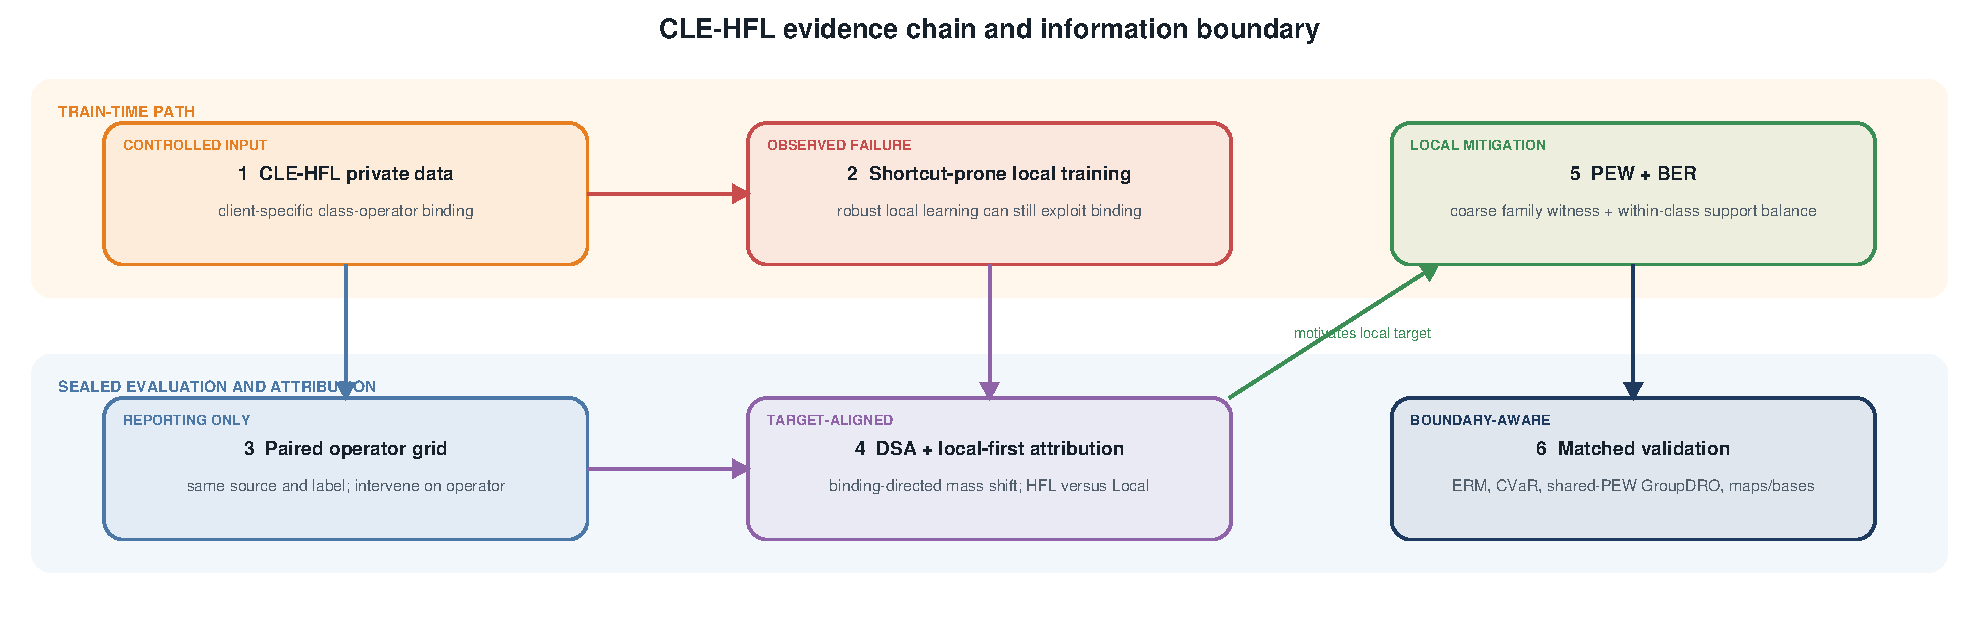
\includegraphics[width=0.98\textwidth]{figures/fig1_cle_hfl_evidence_chain.pdf}
\caption{CLE-HFL evidence chain and information boundary. Training-time PEW+BER uses a coarse family proxy. Operator identities and the binding map are sealed from training and used only for controlled construction or post-training DSA evaluation.}
\label{fig:evidence-chain}
\end{figure*}

\subsection{Axis I: Matched Shortcut-Objective Attribution}

A five-arm 12-round screen was used for method selection only. JTT therefore remains screening-only and is not part of the Formal comparison. Axis I deliberately retains the strong-stress held-out-map2 setting ($\alpha=0.5$, private corruption rate $1.0$, and $\gamma=0.9$) and compares four matched arms: ERM, protocol-matched CVaR-DRO, PEW+GroupDRO, and PEW+BER. They share the same partition, training/evaluation seed, initial states, private batch trajectory, and strict HFL communication protocol. PEW+GroupDRO and PEW+BER receive the same PEW group assignments. Its primary outcome is binding-directed shortcut use measured by DSA; task utility remains reported as a separate outcome rather than hidden or interpreted as ordinary clean-CIFAR performance.

\begin{table*}[t]
\centering
\small
\caption{Held-out map2 matched objective comparison over training seeds 0/1/2 (mean $\pm$ sample standard deviation).}
\label{tab:map2-methods}
\resizebox{\textwidth}{!}{%
\begin{tabular}{lrrrrrr}
\toprule
Arm & DSA $\downarrow$ & Operator-grid Acc. $\uparrow$ & Last-10 Avg $\uparrow$ & Last-10 Worst $\uparrow$ & WCCA $\uparrow$ & CFG $\downarrow$ \\
\midrule
ERM & $0.2505\pm0.0087$ & $20.4950\pm0.3718$ & $19.9589\pm0.1212$ & $16.3780\pm0.1259$ & $0.0000\pm0.0000$ & $32.7467\pm0.1708$ \\
CVaR-DRO & $0.0867\pm0.0055$ & $19.2206\pm1.1055$ & $18.5788\pm0.3102$ & $14.2636\pm0.2640$ & $0.1167\pm0.0629$ & $27.6750\pm0.1885$ \\
\ifdraftskeleton
JTT Formal & \pendingcell & \pendingcell & \pendingcell & \pendingcell & \pendingcell & \pendingcell \\
\fi
PEW+GroupDRO & $0.2054\pm0.0080$ & $21.4517\pm0.5783$ & $20.9963\pm0.0924$ & $17.5309\pm0.5148$ & $0.0333\pm0.0144$ & $31.8950\pm0.9747$ \\
\textbf{PEW+BER} & $\mathbf{0.0715\pm0.0113}$ & $\mathbf{25.1772\pm1.2522}$ & $\mathbf{24.5466\pm0.1098}$ & $\mathbf{20.7516\pm0.6126}$ & $\mathbf{2.6500\pm0.0750}$ & $\mathbf{22.7825\pm0.5428}$ \\
\bottomrule
\end{tabular}%
}
\ifdraftskeleton
\par\smallskip
JTT remains screening-only; an O1 Formal row should be populated only if a formal JTT comparison is later authorized and completed.
\fi
\end{table*}


For training seed 0, the source-paired DSA differences are

\[
\mathrm{DSA(ERM)}-\mathrm{DSA(BER)}=0.182567,
\]

with 95\% interval \([0.180596,0.184407]\),

\[
\mathrm{DSA(GroupDRO)}-\mathrm{DSA(BER)}=0.136834,
\]

with \([0.134952,0.138706]\), and

\[
\mathrm{DSA(BER)}-\mathrm{DSA(CVaR)}=-0.011240,
\]

with \([-0.012355,-0.010092]\). These intervals resample semantic sources conditional on the seed-0 checkpoints.

Across training seeds 0/1/2, DSA(ERM)$-$DSA(BER) is \(0.179060\pm0.008594\), and DSA(GroupDRO)$-$DSA(BER) is \(0.133947\pm0.011518\); both contrasts favor BER in all three seeds. DSA(BER)$-$DSA(CVaR) is \(-0.015184\pm0.015411\), while BER improves operator-grid accuracy over CVaR by \(5.9567\pm2.3151\) percentage points. The pre-registered multi-seed gates pass, yielding \texttt{GO\_MAP2\_TRAINING\_SEED\_STABILITY}.

The shared-PEW comparison separates access to PEW groups from the BER objective: PEW+GroupDRO retains pooled DSA \(0.2054\pm0.0080\), whereas PEW+BER reaches \(0.0715\pm0.0113\). CVaR-DRO is closer at \(0.0867\pm0.0055\), but BER also has higher pooled operator-grid accuracy, Avg, Worst, and WCCA, and lower CFG. Per-client DSA is not uniformly ordered: CVaR-DRO is lower on c0 and c1, while BER is lower on c2 and c3. Among these four matched objectives, PEW+BER therefore gives the best pooled shortcut--utility trade-off on held-out map2 without per-client DSA dominance over CVaR-DRO.

\subsection{Cross-Binding and Cross-Communication Validation}

Table~\ref{tab:cross-setting-dataset} summarizes completed PEW+BER comparisons on the original binding map, map1, and FedDF-fidelity. A second private dataset remains a separate evidence slot.

\begin{table*}[t]
\centering
\small
\caption{Within-setting PEW+BER comparisons across binding maps and communication bases.}
\label{tab:cross-setting-dataset}
\resizebox{\textwidth}{!}{%
\begin{tabular}{lllrrrr}
\toprule
Private task & Binding / protocol & HFL base & Base DSA & PEW+BER DSA & Relative reduction & Avg delta \\
\midrule
CIFAR--10 & original map & Asymmetric HFL & 0.119644 & 0.041252 & 65.52\% & +1.7323 \\
CIFAR--10 & map1 & Asymmetric HFL & 0.113761 & 0.049531 & 56.46\% & +0.7040 \\
CIFAR--10 & held-out map2 (3 seeds) & Asymmetric HFL & 0.250530 & 0.071470 & 71.47\% & +4.5877 \\
CIFAR--10 & original map & FedDF-fidelity & 0.136989 & 0.029012 & 78.82\% & -0.6660 \\
\ifdraftskeleton
Second private task & dataset/protocol pending & pending & \pendingcell & \pendingcell & \pendingcell & \pendingcell \\
\fi
\bottomrule
\end{tabular}%
}
\ifdraftskeleton
\par\smallskip
\evidenceneeded{second private dataset; dataset and protocol pending.}
\fi
\end{table*}


On map1, only the client-specific class--operator binding changes; the partition, evaluation seed, training seed, initial weights, public data, evaluation grid, and frozen PEW remain fixed. Pooled DSA changes from \(0.113761\) to \(0.049531\), a 56.46\% reduction, and all four clients move in the same direction. Operator-grid accuracy changes from \(20.9450\%\) to \(21.4583\%\). This reproduces DSA suppression on a second controlled binding direction at seed 0.

The completed second communication-base experiment uses native single-view CE with a protocol-matched \textbf{FedDF-fidelity} adapter. Base and BER arms share initialization, private batches, public distillation, and training budget. Pooled DSA changes from \(0.136989\) to \(0.029012\), while operator-grid accuracy changes by \(-0.0400\) points and last-five Avg by \(-0.6660\) points. The frozen utility gate fails, and both arms fall below the pre-registered 20\% operator-grid learning floor. We use this experiment as boundary evidence that DSA suppression can appear under another communication mechanism; it does not establish cross-base utility gain.

To test the stronger mechanism-level question under a classic and computationally light communication rule, a pending FedMD replication holds communication fixed across the same four local objectives used in the main comparison. This experiment is a controlled cross-communication replication, not a claim that PEW+BER is universally compatible with every HFL algorithm.

\evidenceneeded{second private dataset; dataset and protocol pending.}

\subsection{Moderate CLE Dose Response and Utility}

The strong-stress protocol intentionally combines severe label skew, corruption of every private image, and strong class--operator binding. It is suitable for mechanism stress testing but can confound low semantic utility with shortcut dependence. A separate, pre-specified moderate protocol keeps the private task and held-out binding map fixed while using Dirichlet $\alpha=1.0$, private corruption rate $\rho=0.5$, and $\gamma\in\{0,0.5,0.9\}$. For sample $i$ at client $k$, a fixed corruption indicator $C_{ki}\sim\mathrm{Bernoulli}(\rho)$ is shared across all three $\gamma$ conditions. Conditional on $C_{ki}=1$,
\[
P(E=e\mid Y=c,k,C=1)=\frac{1-\gamma}{11}+\gamma\mathbf{1}[e=b_k(c)].
\]
Sources, labels, corruption masks, severities, fit/audit splits, model initialization, public data, and the paired operator grid are held fixed. Thus $\alpha$ controls client label support, $\rho$ controls exposure to corruption, and $\gamma$ controls class-conditional operator concentration. This protocol is a second controlled difficulty regime on CIFAR--10, not a second private dataset.

\ifdraftskeleton
\begin{table}[t]
\centering
\small
\caption{Pending moderate-protocol dose response. The corruption mask, partition, sources, severities, initialization, and evaluation grid are paired across $\gamma$.}
\label{tab:moderate-dose}
\resizebox{\columnwidth}{!}{%
\begin{tabular}{llrrrr}
\toprule
$\gamma$ & Objective & DSA $\downarrow$ & Operator Acc. $\uparrow$ & Clean Acc. $\uparrow$ & Avg $\uparrow$ \\
\midrule
0.0 & ERM & \pendingcell & \pendingcell & \pendingcell & \pendingcell \\
0.5 & ERM & \pendingcell & \pendingcell & \pendingcell & \pendingcell \\
0.9 & ERM & \pendingcell & \pendingcell & \pendingcell & \pendingcell \\
0.9 & PEW+BER & \pendingcell & \pendingcell & \pendingcell & \pendingcell \\
\bottomrule
\end{tabular}%
}
\end{table}
\fi


\evidenceneeded{Formal moderate-protocol ERM dose response at gamma 0/0.5/0.9 and matched PEW+BER at gamma 0.9.}

\subsection{Axis II: HFL Mechanism-Family Context}

Axis II asks a different question from the matched objective study: whether representative heterogeneous-FL communication and robustness mechanisms naturally remove CLE while retaining usable task semantics. The pre-specified eight-row main table contains Local/ERM, FedMD, FedProto, FedDF, AugHFL, RAHFL, AsymHFL--ERM, and AsymHFL+PEW+BER. All final rows use the moderate held-out-map2 condition ($\alpha=1.0$, $\rho=0.5$, $\gamma=0.9$), training seed 0, the same 40-round budget, initial states, and paired operator evaluation grid. Ordinary HFL mechanisms and corruption-robust AugHFL/RAHFL are retained because communication robustness, corruption robustness, and directional-shortcut suppression are distinct capabilities. We report DSA together with paired-grid, clean-subset, corrupted-subset, and overall task accuracy; per-client DSA and Worst/WCCA/CFG remain in the detailed analysis. Existing strong-stress Local/FedMD runs are internal engineering records and do not enter the paper tables.

\ifdraftskeleton
\begin{table*}[t]
\centering
\small
\caption{Protocol-matched HFL mechanism-family context on the moderate held-out-map2 protocol ($\alpha=1.0$, private corruption rate $0.5$, and $\gamma=0.9$; Axis II). Scientific metric cells remain pending until the Formal runs are completed and audited.}
\label{tab:hfl-context}
\resizebox{\textwidth}{!}{%
\begin{tabular}{llllrrrrr}
\toprule
Method & Model heterogeneity & Local robustness & Communication & DSA $\downarrow$ & Grid Acc. $\uparrow$ & Clean Acc. $\uparrow$ & Corrupt Acc. $\uparrow$ & Avg $\uparrow$ \\
\midrule
Local/ERM & yes & none & none & \pendingcell & \pendingcell & \pendingcell & \pendingcell & \pendingcell \\
FedMD adapter & yes & none & public-logit exchange & \pendingcell & \pendingcell & \pendingcell & \pendingcell & \pendingcell \\
FedProto adapter & yes & none & class prototypes & \pendingcell & \pendingcell & \pendingcell & \pendingcell & \pendingcell \\
FedDF-fidelity & yes & none & public distillation & \pendingcell & \pendingcell & \pendingcell & \pendingcell & \pendingcell \\
AugHFL-fidelity & yes & AugMix/JSD & heterogeneous collaboration & \pendingcell & \pendingcell & \pendingcell & \pendingcell & \pendingcell \\
RAHFL anchor & yes & AugMix/JSD/DCL & asymmetric collaboration & \pendingcell & \pendingcell & \pendingcell & \pendingcell & \pendingcell \\
AsymHFL--ERM & yes & none & strict asymmetric collaboration & \pendingcell & \pendingcell & \pendingcell & \pendingcell & \pendingcell \\
AsymHFL+PEW+BER & yes & class-conditional environment balancing & strict asymmetric collaboration & \pendingcell & \pendingcell & \pendingcell & \pendingcell & \pendingcell \\
\bottomrule
\end{tabular}%
}
\par\smallskip
The eight-row main table is fixed before results are observed. Existing strong-stress Local/FedMD and all smoke/benchmark outputs are engineering records only and are excluded from the paper table.
\end{table*}
\fi


\evidenceneeded{Formal scientific metrics for the moderate held-out-map2 HFL mechanism-family context table.}

\begin{figure*}[t]
\centering
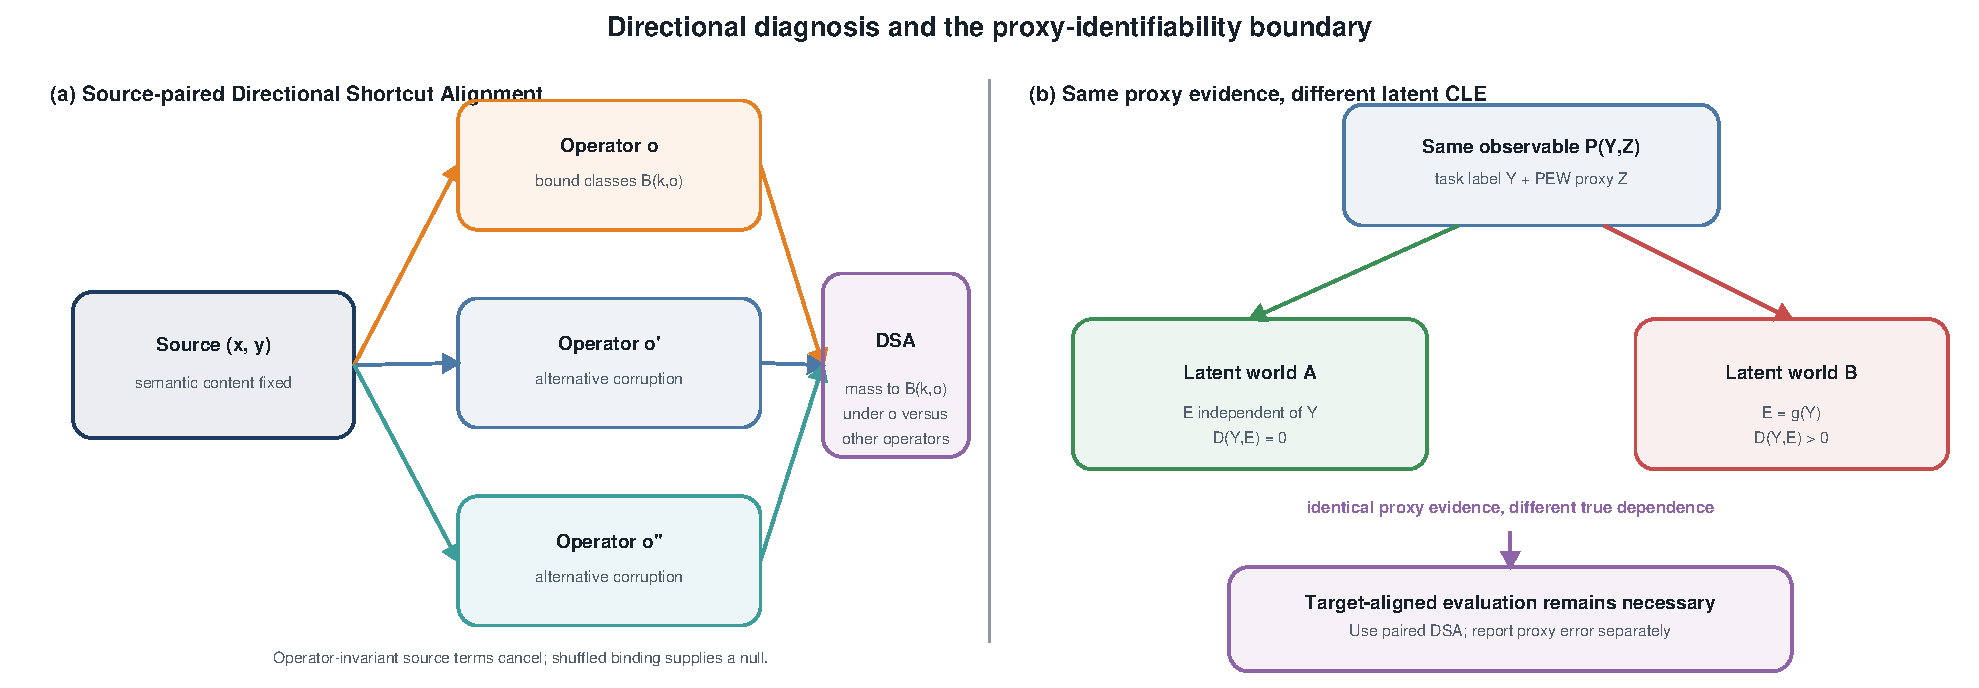
\includegraphics[width=0.98\textwidth]{figures/fig2_dsa_proxy_boundary.pdf}
\caption{Paired directional diagnosis and proxy-identifiability boundary. DSA compares bound-class probability mass across operators for the same source. Identical observable label--proxy evidence can correspond to latent worlds with different true dependence.}
\label{fig:dsa-proxy}
\end{figure*}

\subsection{Environment Correspondence and Granularity}

A non-deployable Oracle audit compares true family grouping, true operator grouping, and a random operator correspondence. Random operator DSA exceeds Oracle operator DSA by \(0.052112\), with source-bootstrap 95\% interval \([0.051231,0.052983]\), showing that the environment correspondence matters in this audit. The Oracle family--operator DSA gap is \(0.001449\), with \([0.001086,0.001790]\). The small granularity gap is specific to this controlled audit and provides no empirical reason to introduce an operator-level PEW in the current paper. Appendix C reports the complete Oracle table.

\subsection{Remaining Evidence Placeholders}

The internal manuscript keeps unresolved evidence visible. The existing three-seed strong-stress held-out-map objective comparison is complete under its frozen protocol; a higher-budget seed-0 repeat is being audited separately and must not be mixed before completion. Remaining experiments are the moderate dose response, the moderate-protocol HFL context table, the multi-seed local-first extension, a genuinely second private dataset, a bounded taxonomy stress test, and the FedMD four-objective replication. A JTT Formal is optional and is needed only if the final paper makes a direct empirical superiority claim over JTT.

\evidenceneeded{local-first training seeds 1/2.}

\evidenceneeded{bounded taxonomy stress test; protocol pending.}
